% KSe.tex
% $Author$ $Date$

% \section{\KSe}
% \label{s-KS}
% Predrag                    4jul2006
% Predrag                   jun 20 2006
% Vaggelis                  may 20 2006
% extracted from ~dasbuch/book/chapter/PDEs.tex  5jun2005 version
% Predrag                   17sep1999

% \PC{incorporate missing refs from chapter/refsPDEs.tex}

The \KS\ [henceforth KS] system\rf{ku,siv},
which arises in the description of
stability of flame fronts, reaction-diffusion systems and many other
physical settings\rf{KNSks90}, is one of the simplest nonlinear PDEs that
exhibit spatiotemporally chaotic behavior. In the formulation
adopted here, the time evolution of the `flame front velocity'
$u=u(x,t)$ on a periodic domain $u(x,t) = u(x+L,t)$ is given by
\beq
  u_t+{\textstyle\frac{1}{2}}(u^2)_x+u_{xx}+ u_{xxxx}=0
% abandoned the CCP convention: u_t=(u^2)_x-u_{xx}- u_{xxxx}
    \,,\qquad   x \in [-L/2,L/2]
    \,.
\ee{ks}
Here $t \geq 0$ is the time, and $x$ is the spatial coordinate.
The subscripts $x$ and $t$ denote partial derivatives with respect to
$x$ and $t$.
% In the literature \refeq{ks} is sometimes written as
% \[ %beq
%     u_t=(u^2)_x-u_{xx}- \nu \, u_{xxxx}
%     \,,\qquad   x \in [0,L]
%     \,,
% \] %\ee{ksVisc}
% or in any number of other variants, all equivalent.
In what follows
we shall state results of all calculations either in units of the
`dimensionless system size' $\tildeL$, or the system size $L = 2 \pi
\tildeL$. %, with the `hyper-viscosity' $\nu$ fixed to $1$. Other
% authors vary  $\nu$, with $L$ fixed to either $1$ or $2\pi$.
All numerical results presented in this paper
are for the system size $\tildeL=22/2\pi = 3.5014\cdots$.
Spatial periodicity $u(x,t)=u(x+L,t)$
makes it convenient to work in the Fourier space,
\beq
  u(x,t)=\sum_{k=-\infty}^{+\infty} a_k (t) e^{ i k x /\tildeL }
\,,
% \label{fseries}
\ee{eq:ksexp}
%where $\tildeL=L/2\pi$. Thus,
with the $1$-dimensional PDE \refeq{ks}
replaced by an infinite set of
ODEs for the complex Fourier coefficients $a_k(t)$:
\beq
\dot{a}_k= \pVeloc_k(a)
     = ( (k/\tildeL)^2 - ( k/\tildeL)^4 )\, a_k
    - i \frac{k}{2\tildeL} \sum_{m=-\infty}^{+\infty} a_m a_{k-m}
\,.
\ee{expan}
Since $u(x,t)$ is real, $a_k=a_{-k}^\ast$, and we can replace the
sum by a $k > 0$ sum.

\PC{find better place for this text?}
Due to the hyperviscous damping $u_{xxxx}$, long time solutions of
\KSe\ are smooth, $a_k$ drop off fast\PC{how fast?} with $k$,
and truncations of \refeq{expan} to $16 \leq d \leq 128$  terms
yield accurate solutions for system sizes considered here.
Robustness of the long-time dynamics of KS as a function of the
number of Fourier modes kept in truncations of \refeq{expan} is, however,
a subtle issue.
Adding an extra mode to a truncation of the system
introduces a small perturbation in the space of dynamical
systems. However, due to the lack
of structural stability both as a function of truncation $d$, and the
system size \tildeL, a small variation in a system parameter
can (and often will) throw the dynamics
into a different asymptotic state.
For example, asymptotic attractor
which appears to be chaotic in a $d$-dimensional
\statesp\ truncation can
collapse into an attractive period-$n$ cycle for
$(d\!+\!1)$-dimensions.

%%%%%%%%%%%%%%%%%%%%%%%%%%%%%%%%%%%%%%%%%%%%%%%%%%%%%%%%%%%%%%
\begin{figure}[t]
\begin{center}
%\includegraphics[width=0.8\textwidth]{figs/ks_largeL.eps}
\includegraphics[width=0.9\textwidth]{figs/ks_largeL_cbar.eps}
\end{center}
\caption{
A typical `turbulent' solution of the \KSe, system size
$L=20\pi\sqrt{2}\approx 88.86$.  The $x$ coordinate is scaled
with the most unstable wavelength $2\pi\sqrt{2}$, which is
approximately also the mean wavelength of the turbulent flow.
The color bar indicates the color scheme for $u(x,t)$.  This color
scheme is used in other figures of this type throughout this work.
     } \label{f:ks_largeL}
\end{figure}
%%%%%%%%%%%%%%%%%%%%%%%%%%%%%%%%%%%%%%%%%%%%%%%%%%%%%%%%%%%%%%%%%%

\subsection{Symmetries of \KSe}
\label{sec:KSeSymm}

The KS equation is Galilean invariant: if $u(x,t)$ is a solution,
then $u(x \PCedit{-ct,t) -c} $, with $c$ an arbitrary constant
speed, is also a solution. Without loss of generality, in our
calculations we shall set the mean velocity of the front to zero,
\beq \int dx \, u = 0 \,. \ee{GalInv}
As $\dot{a_0}=0$ in
\refeq{expan}, $a_0$ is a conserved quantity, in our calculations
fixed to $a_0=0$ by the
% Galilean invariance
condition \refeq{GalInv}.
$G$, the group of actions $ g \in G $
on a \statesp\ (reflections, \PCedit{translations}, \etc)
is a symmetry of the flow
$\dot{u} = F(u)$ if $g\,\dot{u} = F(g\,u)$.
The KS equation % \refeq{ks}, 
\beq
\dot{u} = 
F(u) = -u u_x-u_{xx}- u_{xxxx}
% \,,
\ee{KSO2}
is time
translationally invariant, and space translationally invariant
on a periodic domain under
the 1-parameter group of 
\PCedit{
$O(2): \{\Shift_{\shift/L},\Refl \}$.
       }
If $u(x,t)$ is a solution, then
$\Shift_{\shift/L}\, u(x) = u(x+\shift,t)$
is an equivalent solution for any \PCedit{shift}
$-L/2 < \shift \leq L/2$,
as is the
reflection (`parity' or `inversion')
\beq
    \Refl \, u(x) = -u(-x)
\,.
\ee{KSparity}
The translation operator action on the Fourier coefficients
\beq
  (\Shift_{\shift/L}\, a)_k= e^{ik\, \shift /\tildeL} \, a_k
    \qquad \mbox{(no summation on $k$)}
    \,.
    \label{eq:RPOcondFouri}
\eeq
amounts to the $k$-th mode complex plane rotation by an angle
$-k\, \shift /\tildeL$, and the reflections acts on them
by complex conjugation,
\beq
  \Refl \, a_k = -a_k^\ast
% a_{2m} \to a_{2m}
\,.
\ee{FModInvSymm}
Reflection generates the dihedral subgroup $D_1 = \{1, \Refl\}$ 
of $O(2)$.  Let $\bbU$ be the space of
real-valued velocity fields periodic and square integrable
on the interval $\Omega = [-L/2,L/2]$,
\begin{align}
 \bbU  &= \{u \in L^2(\Omega) \; | \; u(x) = u(x+L)\}  \,.
\end{align}
A continuous symmetry maps each state $u \in \bbU$ 
to a manifold of functions with identical dynamic behavior.
Relation $\Refl^2 = 1$ induces linear decomposition
$u(x) = u^+(x)+ u^-(x)$, 
\PCedit{
$u^\pm(x)= P^\pm u(x) \in  \bbU^\pm$,
into irreducible subspaces
$
\bbU = \bbU^+  % \oplus  \bbUsymm
       \oplus \bbU^-
$, where
        }
\beq
    P^+=(\matId+\Refl)/2
    \,,\qquad
    P^-=(\matId-\Refl)/2
\ee{P1P2proj}
are the antisymmetric/symmetric projection operators.
Applying $P^+,\,P^-$ on the KS equation \refeq{KSO2}
we have\rf{KNSks90}
\bea
 u_t^+ &=& - (u^+u^+_x + u^-u^-_x )
                - u^+_{xx} - u^+_{xxxx}
    \continue
 u_t^- &=& - (u^+u^-_x + u^-u^+_x )
                - u^-_{xx} - u^-_{xxxx}
\,.
\label{KSD1}
\eea
If $u^- = 0$, KS flow is confined to
the antisymmetric $\bbU^+$ subspace,
\beq
 u_t^+ = - u^+u^+_x
                - u^+_{xx} - u^+_{xxxx}
%        \,,\qquad   x \in
\,,
\label{KSU+}
\eeq
but otherwise the nonlinear terms in \refeq{KSD1}
mix the two subspaces.
    \PC{still to be incorporated, most likely in the next paper:
    wrote down \refeq{KSD1} in order to (a) to clarify embedding of
    $\bbU^+$ into $\bbU$
    (b) to explain the desymmetrization of evolution defined on
     $\Omega^{+} = [0, L/2]$ fundamental domain, with evolution at
    instant of crossing $x=0$ given by reflection $\Refl$.
    Re integrators: make sure $\Refl$ applied after
    all points used by integrator are in $\bbU^-$
    }


Together with any rational shift
$ \Shift_{1/m}u(x)=u(x+L/m)$
reflection generates a discrete dihedral $D_m$
subgroup of $O(2)$, also a symmetry of KS.
The only non-zero Fourier components of a solution invariant
under $D_m$ are $a_{jm} \neq 0$, $j =1,2,\cdots$ .
$D_m$ reduces the dimensionality
of \statesp\ and aids computation of \eqva\ and \po s
within it. For example, the 1/2-cell translations 
\ES{moved all references to 1/2-cell translation to one place.}
\beq
    \Shift_{1/2}\, u(x)=u(x+L/2)
\,,
\ee{KSshift}
and reflections generate $O(2)$
subgroup $D_2 = \{1, \Refl,\Shift,\Shift\Refl\}$,
which
reduces the \statesp\ into four irreducible subspaces
(for brevity, here $\Shift = \Shift_{1/2}$):
\PC{dangerous edit, changed $S \to A$ for reflections,
    please cross-check}
\PCedit{
\begin{align}
 & \qquad\qquad\qquad\qquad\qquad
              ~~~ \Shift ~~ \Refl  ~\;  \Shift\Refl
    \nnu\\
P^{(1)} &= \frac{1}{4} (1 + \Shift + \Refl + \Shift\Refl)
           ~~~~  S  ~~  A   ~~   A
    \nnu\\
P^{(2)} &= \frac{1}{4} (1 + \Shift - \Refl - \Shift\Refl)
            ~~~~  S  ~~  S   ~~   S
    \nnu\\
P^{(3)} &= \frac{1}{4} (1 - \Shift + \Refl - \Shift\Refl)
           ~~~~  A  ~~  A   ~~   S
     \label{ek_defn}\\
P^{(4)} &= \frac{1}{4} (1 - \Shift - \Refl + \Shift\Refl)
          ~~~~  A  ~~  S   ~~   A
\,.
    \nnu
\end{align}
        }
$P^{(j)}$ is the projection operator onto
$u^{(j)}$ irreducible subspace, and the last 3 columns
refer to the symmetry of
$u^{(j)}$ functions under reflection and
1/2-cell shift.
By the same argument that identified \refeq{KSU+} as
the invariant subspace of KS, here the KS flow
stays within the  
\PCedit{
 $\bbU^S =  \bbU^{(1)}+ \bbU^{(2)}$ 
irreducible $D_1$ subspace of $\bbU$
       } 
profiles symmetric under 1/2-cell shifts.

    \PC{abandoned the \refref{KNSks90} notation, I might be wrong,
        please recheck. Replace $\mathbf{L} \to P^{(1)}$ downstream}
\PCedit{
While in general the bilinear term $(u^2)_x$  mixes the
irreducible subspaces of $D_n$, for $D_2$ there are
four subspaces invariant under the flow\rf{KNSks90}:
\begin{romannum} % SIAM itemize}
 \item[$\{0\}$:~~~~~~] the $u(x)=0$ {\eqv}
 \item[$\bbU^+ = \bbU^{(1)}+ \bbU^{(3)} $:] 
    the reflection $D_1$ irreducible space of antisymmetric $u(x)$
 \item[$\bbU^S =  \bbU^{(1)}+ \bbU^{(2)}$:] 
    the shift $D_1$ irreducible space of $L/2$ shift symmetric  $u(x)$
 \item[$\bbU^{(1)}$:~~~~~]
    the $D_2$ irreducible  space of $u(x)$ invariant under $x\mapsto L/2-x,\ u\mapsto -u$
\end{romannum} %itemize}
as long as all other components of $u(x)$ are 
set to zero (see for example \refeq{KSU+}).
        } % end \PCedit
With the continuous
translational symmetry eliminated within each subspace, there are no
\reqva\ and \rpo s, and one
can focus on the \eqva\ and \po s only, as was done
for $\bbU^+$ in \refrefs{Christiansen:97,Lan:Thesis,LanCvi07}.
In the Fourier
representation, the 
\PCedit{
$u \in \bbU^+$
    }
antisymmetry amounts to having purely imaginary
coefficients, since $a_{-k}= a^\ast_k = -a_k$.
The 1/2 cell-size shift $\Shift_{1/2}$
generated 2-element discrete subgroup
$\{1,\Shift_{1/2}\}$ is
of particular interest
because in the 
\PCedit{
$\bbU^+$
       }
subspace the translational invariance of the full system reduces to
invariance under discrete translation \refeq{KSshift} by half a
spatial period $L/2$.

Each of the above dynamically invariant subspaces is unstable
under small perturbations, and generic solutions of \KSe\ belong to
the full space.
Nevertheless, since  all \eqva\ of the KS flow studied in this paper
lie in the $\bbU^+$ subspace (see
\refsect{sec:L22}), $\bbU^+$  plays important role for the global
geometry of the flow.
However, linearized stability of these \eqva\ has
eigenvectors both in and outside of $\bbU^+$, and needs to be
computed in the full \statesp.
% via four products $\Refl_{1,2} \Shift_{1,2}$



\subsection{\Eqva\ and \reqva} % of the \KSe}
\label{sec:stks}
% former equilibria.tex

% Predrag                   jun 20 2006
% Vaggelis                  may 20 2006
% Predrag                                       05dec2004
% Lan                                           25nov2004
% from Lan thesis                                8jun2004

\Eqva\  (or the steady solutions)
are the fixed profile time-invariant solutions,
\beq
 u(x,t) = u_\stagn(x) %\,,\quad t \in \mathbb{R}
\,.
\ee{eqva}
Due to the translational symmetry,
the KS system also allows for 
\reqva\ (traveling waves, rotating waves),
characterized by a fixed profile $u_\stagn(x)$
moving with constant speed $c$, {\ie}
\beq
 u(x,t) =  u_\stagn(x-ct) %\,,\quad t \in \mathbb{R}
\,.
\ee{reqva}
Here suffix ${}_\stagn$ labels a particular invariant solution.
Because of the reflection symmetry \refeq{KSparity},
the \reqva\ come in counter-traveling pairs
$u_\stagn(x-ct)$, $-u_\stagn(-x+ct)$.

The \reqv\ condition for the {\KS} PDE \refeq{ks}
is the ODE
\beq
{\textstyle\frac{1}{2}}(u^2)_x+u_{xx}+ u_{xxxx}=c \, u_x
% \,.
\ee{KSeqvCond}
which can be analyzed as a dynamical system in its own right.
\PC{\PCedit{PC: please recheck $E$ vs $c$}}
Integrating once we get
\PC{
    \reqva\ = \eqva\ shifted by $c$?
   }
\ESedit{
\beq
{\textstyle\frac{1}{2}}u^2 - c u + u_x + u_{xxx}=\expctE
\,.
\label{eq:stdks}
\eeq
}%End ESedit
The integration constant \expctE\ can be interpreted as `energy',
see \refsect{sec:energy}.
% Integrate over $L$, and $u_x$, $u_{xx}$ drop put by the
% $L$ periodicity.
Written as a 3-dimen\-si\-on\-al dynamical system
with spatial coordinate $x$ playing the role of `time',
%\refeq{eq:stdks}
this is a volume preserving flow
\beq
\ESedit{
v = u_x \,,\qquad
w = v_x \,,\qquad
w_x = \expctE - {\textstyle\frac{1}{2}} u^2 + c u - v 
       }% end ESedit
\,,
  \label{eq:3dks}
\eeq
\ES{
Changed signs here, seemed simpler this way. 
PC: I remember having a reason, so something down the line 
    came out with consistent signs. Perhaps \refeq{eqvOfEqv}?
   }
with the `time' reversal symmetry,
\[
x \to -x,\quad u \to -u, \quad v \to v, \quad w \to -w \,.
\]
    \ES{
   The term $c u$ breaks the symmetry. 
   We may overcome this by changing sign of c as well, 
   but it is a parameter, not a variable.
       }
\PC{might move space average def \refeq{rpo:spac_ave} to here,
    note that
    $\expct{u} = \expct{v} = \expct{w} =0$
    }
 Rewriting \refeq{eq:3dks} as 
     \ES{With the corrected form of \refeq{eq:stdks} we cannot write this}
\beq
\PCedit{
(u+w)_x={\textstyle\frac{1}{2}}(u-c)^2-\expctE
    ={\textstyle\frac{1}{2}}(u-c-\sqrt{2\expctE}) (u-c+\sqrt{2\expctE})
       } %end \PCedit{
\ee{eqvOfEqv}
we see that
for $\expctE<0$, 
    \ES{Isn't $E>0$ by definition?
    PC: Here $E$ is an integration constant - do not see how
    we can argue $E \geq 0$ at this point.
        } 
$u+w$ increases without bound with $x \to \infty$,
and every solution escapes to infinity.
If $\expctE=0$, the origin $(0,0,0)$ is the
only bounded  solution, a marginally stable center with
eigenvalues $(0, i,-i)$.

For $\expctE>0$ there is rich
$\expctE$-dependent dynamics, with
fractal sets of bounded solutions investigated in
depth by Michelson\rf{Mks86}.
%
% former\subsection{Bifurcation structure of \eqva\ and \reqva.}
% \label{sec:KSlit}
% Vaggelis               jan 20 2007
%
For $\tildeL<1$ the only \eqv\ of the system is the
globally attracting constant
solution $u(x,t)=0$, denoted $\EQV{0}$ from now on. With increasing system size $L$ system
undergoes a series of bifurcations.
The resulting \eqva\ and
\reqva\ (but not \po s and \rpo s)
are described in the classical papers of
Kevrekidis, Nicolaenko and Scovel\rf{KNSks90},
and Greene and Kim\rf{ksgreene88},
The relevant bifurcations
up to the system size
investigated here are summarized
in \reffig{fig:ksBifDiag}:
at $\tildeL=22/2\pi =
3.5014\cdots$, the {\eqva} are the constant solution
\EQV{0}, the GLMRT\rf{laquey74,ksgreene88} \eqv\ \EQV{1}, the $2$-
and $3$-cell states \EQV{2} and \EQV{3}, the pair of \reqva\
\REQV{\pm}{1}, and the  \REQV{\pm}{2} \reqva.

%%%%%%%%%%%%%%%%%%%%%%%%%%%%%%%%%%%%%%%%%%%%%%%%%%%%%%%%%%%%%%%%
\begin{figure}[t]       \label{fig:ksBifDiag}
\begin{center}
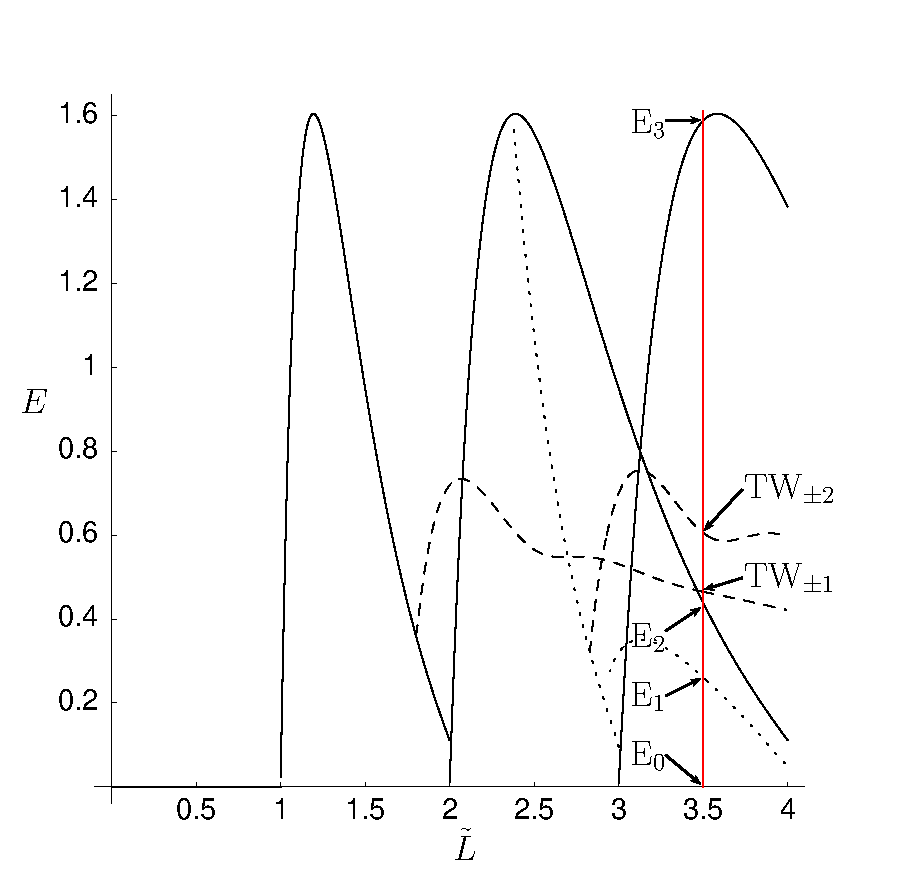
\includegraphics[width=0.5\textwidth]{figs/ksBifDiag_pst.eps}
\end{center}
\caption{
The energy \refeq{ksEnergy} of the \eqva\ and \reqva\ that
exist up to $L=22$, $\tildeL = 3.5014\cdots$, plotted as a function
of the system size $\tildeL = L/2\pi$ (additional \eqva, not present
at $L = 22$ are given in \refref{ksgreene88}). Solid curves denote
$n$-cell solutions \EQV{2} and \EQV{3}, dotted curves the GLMRT
\eqv\ \EQV{1},
% the dash-dotted curve the `giant states' (??? don't have those),
and dashed curves the \reqva\ \REQV{\pm}{1} and \REQV{\pm}{2}.
The parameter $\alpha$ of \refrefs{KNSks90,ksgreene88} is
related to the system size by $\tildeL=\sqrt{\alpha/4}$.
% Open circles indicate Hopf bifurcations.
%The color of a branch indicates the number of unstable eigenvalues:
%(red) 2 unstable eigenvalues, (blue) 1 unstable eigenvalue, (green)
%stable.
        }
\end{figure}
%%%%%%%%%%%%%%%%%%%%%%%%%%%%%%%%%%%%%%%%%%%%%%%%%%%%%%%%%%%%%%%%%%

\ES{Removed text about equilibria of equilibria.}
% ES removed
%%%%%%%%%%%%%%%%%%%%%%%%%%%%%%%%%%%%%%%%%%%%%%%%%%%%%%5
% The solutions of the {\eqv}  condition
% \refeq{eq:3dks} are
% % themselves in turn
% organized\rf{Mks86} by the
% `{\eqva}  of {\eqva}'  condition
% \( u_x= v_x= w_x= 0 \).
% % , and the connections between them.
%     For $\expctE>0$ the {\reqva}  points of \refeq{eqvOfEqv} are
% $C_{+}=(c+\sqrt{2\expctE},0,0)$ and $C_{-}=(c-\sqrt{2\expctE},0,0)$.
% Linearization of the flow around $C_{+}$ yields the cubic equation
% $ %  \beq
% \eigExp(1+\eigExp^2) = 4 \expctE
% \,,
% $ %  \ee{KSeqvCubic}
% with linear stability eigenvalues
% \beq
% \eigExp[1] = 2 \eigRe
%     \,,\qquad
% \eigExp[2,3] = - \eigRe \pm i \eigIm
% \ee{eqvEqvEigV}
% Hence $C_{+}$ has a {1\dmn}
% unstable manifold and a 2\dmn\ stable manifold
% along which solutions spiral in.
% By the $x \to -x$ `time reversal' symmetry, the
% invariant manifolds of $C_{-}$
% have reversed stability properties.
% \PC{
%     not sure we need this, not used in our paper? Where did the figure go?
%     }
% Most orbits escape quickly even if initiated close to \eqva, and that
% renders the numerical calculations
% difficult\rf{ksham95,kshooper88,pimyk,pimsimp}.
% In this context the variational method
% developed in \refrefs{lanVar1,CvitLanCrete02}
% appears more robust than
% the earlier approaches.
%%%%%%%%%%%%%%%%%%%%%%%%%%%%%%%%%%
% end ES removed

%\subsection{\Eqva\ on a periodic domain}
%

%\RLD{This paragraph should probably be moved down after real-space
%equation for equilibria and traveling waves are discussed.}
In the Fourier representation the \reqva\ time
dependence is
\beq
 a_k(t) e^{-itc k/\tildeL} = a_k(0)
\,.
\ee{reqvaF}
Differentiating with respect to time, we obtain
the Fourier space version of the \reqv\ condition
\beq
 \pVeloc_k(a) - i \frac{k c}{\tildeL} a_k = 0
\,,
\ee{reqvCondF}
which needs to be solved for (time independent) $a_k$ and $c$.
For a periodic boundary cell of size
$L$ the only {\eqva}  are
solutions of \refeq{eq:3dks} of spatial periodicity $L$.
Periods of spatially periodic {\eqva} are multiples of $L$.
Every time the system size crosses  $\tildeL=n$,
$n$-cell states
are generated through pitchfork bifurcations off $u =0$
equilibrium.
Due to the translational invariance of {\KSe},
they form invariant circles
in the full \statesp.
In the discrete symmetry subspace considered here,
they correspond to two points, one $L/2$ shift of the other.

For any fixed period $L$ the number
of spatially periodic solutions is finite up to a spatial translation.
For a sufficiently small $L$
the number of {\eqva} is small and
concentrated on the low wave-number end of the Fourier spectrum.

In a periodic box of size $L$
both \eqva\ and \reqva\ are  periodic solutions
embedded in 3-$d$ space \refeq{eq:3dks},
conveniently represented as loops in
$(u,v,w)$ space \ES{dropped 
whose topology is controlled by the
`\eqva\ of \eqva' stable-unstable manifold structure of
\refeq{eqvEqvEigV} }
, see \reffig{f:KS22Equil}\,(\textit{d}).
In this representation the continuous translation symmetry
is automatic - a rotation in the $[0,L]$ periodic domain only
moves the points along the loop. For an \eqv\ the points
are stationary in time; for \reqv\ they move in time, but in
either case, the loop remains invariant.
So we do not have the problem that we encounter in the Fourier
representation, where from the frame of one of the \eqva\
the rest trace out circles under the action of continuous symmetry
translations.


\subsection{Stability of \eqva}
\label{s:StabEqui}
%%
% Predrag           5jun2005
% extracted from \Chapter{stability}{ 2apr2005}

If $u_\stagn(x)$ is an \eqv\ solution of \KSe,
the {\stabmat}
${\Mvar}={\Mvar}(a_\stagn)$
is constant in time,
and
the {\jacobianM}
of the \eqv\ solution is
\beq
 \jMps^t(a_\stagn) = e^{{\Mvar} t}
    \,,\qquad
 \Mvar_{ij}= \Mvar_{ij}(a_\stagn)
\,.
\ee{eqvFundMat}
Calculation of the {\stabmat} requires a bit of care:
% \refeq{DerMatrix}
$a_{k}$ cannot be varied independently of $a_{-k}$, as
% \refeq{expan}
the reality of $u(x,t)$ implies that $a_{k}=a^*_{-k}$.
We impose the reality constraint by splitting \refeq{expan}
in real and imaginary parts, $a_k=b_k+i\, c_k$. {\Stabmat}
is then:
% \index{Kuramoto-Sivashinsky system}
\bea
    \frac{\partial \dot{c}_k}{\partial c_{j}} & = &
    \frac{k^2}{\tildeL^2}\left(1- \frac{k^2}{\tildeL^2} \right)\delta_{kj}
    - \frac{k}{\tildeL} (c_{k+j}-c_{k-j})
\continue
    \frac{\partial \dot{c}_k}{\partial b_{j}} & = &
    - \frac{k}{\tildeL} ( b_{k+j}+b_{k-j} )
\label{expanMvar}\\
    \frac{\partial \dot{b}_k}{\partial b_{j}} & = &
    \frac{k^2}{\tildeL^2}\left(1- \frac{k^2}{\tildeL^2} \right)\delta_{kj}
    +  \frac{k}{\tildeL} (c_{k+j} + c_{k-j})
\continue
    \frac{\partial \dot{b}_k}{\partial c_{j}} & = &
    - \frac{k}{\tildeL} (b_{k+j}-b_{k-j})
    \,,\qquad  k,j>0
\,.
\nnu
\eea
For the \KSe\ the constant solution $u(x,t)=0$ with zero energy $E$ is an
\eqv\ point of \refeq{ks} which we shall henceforth refer to as
\EQV{0}. For this `laminar' \eqv\ the {\stabmat}
is diagonal, and
so is the {\jacobianM}
$
\jMps^t_{kj}(0) = \delta_{kj} e^{(k/\tildeL)^2(1- (k/\tildeL)^2)t}
\,.
$

From \refeq{expan} we see that the origin $u(x,t) = 0$
has Fourier modes as the linear stability eigenvectors.
The $|k|<\tildeL$
long wavelength perturbations of the flat-front {\eqv}
are linearly unstable, while all
$|k|> \tildeL$ short wavelength perturbations are strongly contractive.
The high $k$ eigenvalues, corresponding to rapid variations of
the flame front, decay so fast that the corresponding eigendirections
are physically irrelevant.
The most unstable mode, nearest to $|k|=\tildeL/\sqrt{2}$,
sets the scale of the mean wavelength $\sqrt{2}$
of the KS `turbulent' dynamics,
% measured in the system size \tildeL,
see \reffig{f:ks_largeL}.

\subsection{\Rpo s, symmetries and \po s} \label{sec:KSePO}
% Predrag created file              jul 3 2006

The KS equation \refeq{ks} is time translationally invariant,
and space translationally invariant
under the 1-$d$ Lie group of $O(2)$ rotations: if
$u(x,t)$ is a solution, then $u(x+\shift,t)$ and
$-u(-x+\shift,t)$ are equivalent
solutions for any $-L/2 < \shift \leq L/2$.
As a result, KS can have
%\reqva\ (traveling wave) solutions $u(x-ct)$ and
\rpo\ solutions with period $\period{}$ and
a nonzero shift $\shift$, without or with reflection,
\beq
u(x+\shift,\period{}) = u(x,0)
\,,\qquad \mbox{or } \quad
-u(-x+\shift,\period{}) = u(x,0)
\,,
\ee{KSrpos}
\ie, a profile $u(x,0)$ that occurs again after time $\period{}$,
but shifted by $\shift$, and possibly reflected by $\Refl$.
{\Rpo s} are periodic in $c=\shift/\period{}$
co-rotating frame,
but in the stationary frame their trajectories
are quasiperiodic.
Due to the reflection symmetry \refeq{KSparity} of KS equation,
every {\rpo}
$u(x,t)$ with shift $\shift$ has a symmetric partner
$-u(-x,t)$ with shift $-\shift$.

Our search for \rpo s in KS system were
inspired by Vanessa L{\'o}pez\rf{lop05rel} investigation
of {\rpo s} of the Complex Ginzburg-Landau equation.
However, there is a vast literature on
{\rpo s} since their first appearance,
in  Poincar\'e study of
the 3-body problem\rf{ChencinerLink,rtb} where
the Lagrange points are the \reqva.
They arise in dynamics of systems
with continuous symmetries, such as motions of rigid bodies, gravitational
$N$-body problems, molecules and nonlinear waves.
Very recently Viswanath\rf{Visw07b} % arXiv.org/physics/0604062
has found both \reqva\ and \rpo s in the plane Couette problem.

% PC merged this with \rpo s:
% \subsection{Discrete symmetries imply \po s}

As $\shift$ is continuous in the interval $[-L/2, L/2]$,
the likelihood of a $\shift=0$ shift is zero,
unless an exact periodicity is enforced by a discrete symmetry,
such as the dihedral symmetries discussed above.
If the shift $\shift$ of a \rpo\ with period $\period{}$ is such
that $\shift /L$ is a rational number, then the orbit is
periodic with period $n\period{}$.
Due to the KS equation invariance
under reflection \refeq{KSparity},
two types of \po s are possible:

{\bf (a)} The \po\ lies within the  $\bbU^-$ antisymmetric subspace
$-u(-x,0) = u(x,0)$ and $u(x,\period{}) = u(x,0)$.

{\bf (b)} The \rpo\ in \refeq{KSrpos} is of  reflection type
$\Refl\tau_{\shift/L} u(x,\period{}) = u(x,0)$.
%    \RLD{
%    Maybe we should use symmetry operators throughout the discussion?
%The general idea is that in chaotic systems with symmetries we should
%generalize the notion of a periodic solution from $u(\period{}) = u(0)$
%to $u(\period{}) = {\bf S} u(0)$, where ${\bf S}$ is any symmetry
%a solution of the system might posses.
%\\
%PC: good idea
%    }
In the next period $\period{}$ such orbit
reverses its drift,
$\Refl\tau_{\shift/L} u(-x-\shift,2\period{}) = u(x,0)$, and any
shift acquired during time $0$ to
$\period{}$ is compensated by the opposite shift during
evolution from $\period{}$ to $2\period{}$.
%\[
%u(x,\period{}) = \Refl u(x,\period{}/2) =
%   \Refl^2 u(x,0) = u(x,0)
%   \,.
%\]
\Po s built from repetitions of such shorter segments
are encountered in dynamical systems with discrete
symmetries\rf{CvitaEckardt,DasBuch}.
    \PC{
        are there
        {\bf (c)} \po s which have $D_m$ symmetries?
        }
